\chapter{Metodología}\label{cap:metodologia}

Este capítulo describe el diseño experimental completo: los datos y sus etiquetas
(Sección \ref{sec:datos}), la partición temporal y la razón para excluir el periodo del
cierre del mercado (Sección \ref{sec:particion}), los escenarios de desbalance
(Sección \ref{sec:escenarios}), el entrenamiento de los modelos (Sección \ref{sec:entrenamiento}),
los explicadores (Sección \ref{sec:explicadores}), las medidas de estabilidad
(Sección \ref{sec:medidas}), el control de pesos aleatorios (Sección \ref{sec:control}) y las
pruebas estadísticas (Sección \ref{sec:estadistica}). La Figura \ref{fig:flujo} muestra el
flujo completo y la Tabla \ref{tab:diseno} resume los factores.

\begin{table}[ht]
\centering
\caption{Factores del diseño experimental. Cada combinación se entrena con tres semillas de
modelo, lo que da $4 \times 6 \times 3 \times 3 = 216$ modelos.}
\label{tab:diseno}
\small
\begin{tabularx}{\textwidth}{lX}
\toprule
Factor & Niveles \\
\midrule
Arquitectura & GCN, GraphSAGE, GAT, TAGCN \\
Escenario de desbalance & Nativo (1:41,1), 1:10, 1:20, 1:10 con SMOTE, 1:100, 1:200 \\
Compensación & Sin ajuste, pesos por clase, \textit{focal loss} \\
Semilla del modelo & 42, 43, 44 \\
Explicador & GNNExplainer, PGExplainer, Shapley por muestreo, Integrated Gradients,
Expected Gradients \\
Medida de estabilidad & Spearman sobre las 165 variables (principal), Spearman sobre las
variables distintas de cero, Jaccard de las 10 variables principales \\
\bottomrule
\end{tabularx}
\end{table}

\begin{figure}[ht]
\centering
\small
\begin{tikzpicture}[
  caja/.style={draw, rounded corners=2pt, align=center, minimum height=1.05cm,
               text width=2.55cm, fill=black!4, font=\footnotesize},
  flecha/.style={-{Latex[length=2mm]}, thick}]
\node[caja] (d) at (0,0) {Elliptic\\ 203.769 transacciones\\ etiquetas: modo C};
\node[caja] (p) at (3.3,0) {Partición sin el cierre\\ 1--29 / 30--35 / 36--42};
\node[caja] (e) at (6.6,0) {6 escenarios de desbalance (solo entrenamiento)};
\node[caja] (h) at (9.9,0) {Búsqueda de hiperparámetros\\ 8 ensayos, PR-AUC val.};
\node[caja] (m) at (9.9,-2.1) {216 modelos\\ 4 arq. $\times$ 3 pérdidas\\ $\times$ 3 semillas};
\node[caja] (r) at (6.6,-2.1) {Rendimiento\\ PR-AUC, ROC-AUC,\\ filtro de calidad};
\node[caja] (x) at (3.3,-2.1) {5 explicadores\\ 30 ilícitas de val.\\ 5 réplicas};
\node[caja] (s) at (0,-2.1) {Estabilidad: 3 medidas\\ control de pesos\\ aleatorios, pruebas};
\draw[flecha] (d) -- (p); \draw[flecha] (p) -- (e); \draw[flecha] (e) -- (h);
\draw[flecha] (h) -- (m); \draw[flecha] (m) -- (r); \draw[flecha] (r) -- (x);
\draw[flecha] (x) -- (s);
\end{tikzpicture}
\caption{Flujo experimental de la corrida principal.}
\label{fig:flujo}
\end{figure}

\section{Datos}\label{sec:datos}

Se usa el conjunto de datos Elliptic \cite{Weber2019Elliptic}, un grafo de 203.769
transacciones de Bitcoin unidas por 234.355 aristas dirigidas, que representan flujos de fondos
entre transacciones. Cada transacción tiene 165 variables numéricas anonimizadas: 93 describen
la propia transacción (montos, número de entradas y salidas, comisiones y otras) y 72 agregan
información de sus vecinas a uno y dos saltos. Además, cada transacción pertenece a uno de 49
pasos de tiempo, separados aproximadamente dos semanas entre sí, y no hay aristas entre pasos
distintos. Los autores
no publican el significado de las variables.

Las etiquetas son tres: 4.545 transacciones ilícitas (2,2~\%), 42.019 lícitas (20,6~\%) y
157.205 sin etiqueta (77,1~\%). Como clase positiva se toma la ilícita. Como clase negativa
se toman las lícitas y las sin etiqueta juntas. Esta elección reproduce la situación de un
sistema real, en el que la inmensa mayoría de las transacciones no ha sido revisada por nadie
y no se puede descartar que haya ilícitas entre ellas. Con ella, la razón entre negativas e
ilícitas en el entrenamiento es de 41 a 1, que es el desbalance real del problema. La
alternativa de usar solo las lícitas como negativas da una razón de 7,6 a 1 y produce un
problema más fácil y menos realista.

Las variables se escalan con la mediana y el rango intercuartílico, ajustados solo con las
transacciones del periodo de entrenamiento, para que los valores extremos de los montos no
dominen. Una consecuencia de este escalado, que resulta importante para la medición de la
estabilidad, es que toda variable igual a su mediana queda exactamente en cero. En las 30
transacciones que se explican (Sección \ref{sec:explicadores}), en promedio el 44~\% de las
variables vale cero, y la mediana de variables distintas de cero por transacción es 89 de
165.

\section{Análisis exploratorio del grafo}\label{sec:eda}

El grafo es muy disperso (Figura \ref{fig:eda}a). Cada transacción tiene en promedio 2,3
aristas y la mediana es 2; el 34,5~\% de las transacciones tiene una sola arista, y la de mayor
grado tiene 473. Las ilícitas tienen menos conexiones que las lícitas (mediana 1 frente a 2;
media 2,0 frente a 3,1). Ninguna arista une transacciones de pasos de tiempo distintos, de modo
que cada paso es un grafo separado, con entre 1.089 y 7.880 transacciones.

\begin{figure}[ht]
\centering
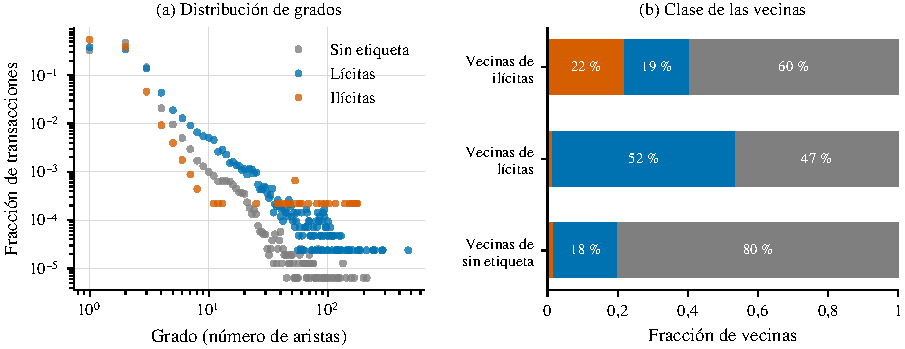
\includegraphics[width=\textwidth]{eda_grafo}
\caption{(a) Distribución del número de aristas por transacción según su clase, en escala
logarítmica. (b) Clase de las vecinas de las transacciones de cada clase, contando cada arista
desde sus dos extremos.}
\label{fig:eda}
\end{figure}

La homofilia de aristas entre transacciones etiquetadas es alta, 0,954, pero está dominada por
las aristas entre lícitas, que son la gran mayoría. La composición de las vecinas de las
ilícitas cuenta otra historia (Figura \ref{fig:eda}b): solo el 21,8~\% de las vecinas de una
transacción ilícita es ilícita, el 18,5~\% es lícita y el 59,6~\% no tiene etiqueta. Visto por
transacción, el 70~\% de las ilícitas no tiene ninguna vecina ilícita. En la tarea de esta tesis,
en la que las transacciones sin etiqueta cuentan como negativas, una ilícita está rodeada sobre
todo de negativas. La señal del fraude, por tanto, está principalmente en las variables de la
propia transacción, y una arquitectura que la promedia con sus vecinas sin darle un peso propio
la diluye (Sección \ref{sec:propiedades}). Este rasgo anticipa el bajo rendimiento de GCN.

\section{Partición temporal y exclusión del cierre del mercado}\label{sec:particion}

La partición respeta el orden del tiempo: el modelo se entrena con los pasos más antiguos y
se evalúa con los más recientes, de modo que nunca ve el futuro. La partición habitual en la
literatura usa los pasos 1 a 34 para entrenar y los pasos 35 a 49 para evaluar, y en este
trabajo se dividió esa evaluación en validación (35 a 42) y prueba (43 a 49).

En el paso 43 se cerró un mercado ilegal importante, y los autores de Elliptic reportaron que
desde ese momento ningún modelo detectaba las nuevas transacciones ilícitas
\cite{Weber2019Elliptic}. Es un cambio en la distribución de los datos a lo largo del tiempo
\cite{Gama2014Drift}: lo que el modelo aprendió de los mercados que existían deja de describir
la actividad ilícita posterior. Con la partición habitual, la prueba completa cae después del
cierre. En la corrida de esta tesis con esa partición, el mejor modelo de cada arquitectura
obtuvo en prueba un PR-AUC entre 0,005 y 0,012, frente a 0,006 que obtendría un clasificador
al azar (Anexo \ref{anx:original}).

Por ello el estudio principal usa solo los pasos 1 a 42 y los reparte en tres bloques
contiguos: entrenamiento con los pasos 1 a 29, validación con los pasos 30 a 35 y prueba con
los pasos 36 a 42 (Figura \ref{fig:particion} y Tabla \ref{tab:particion}). Los pasos 43 a 49
no se usan.

\begin{figure}[ht]
\centering
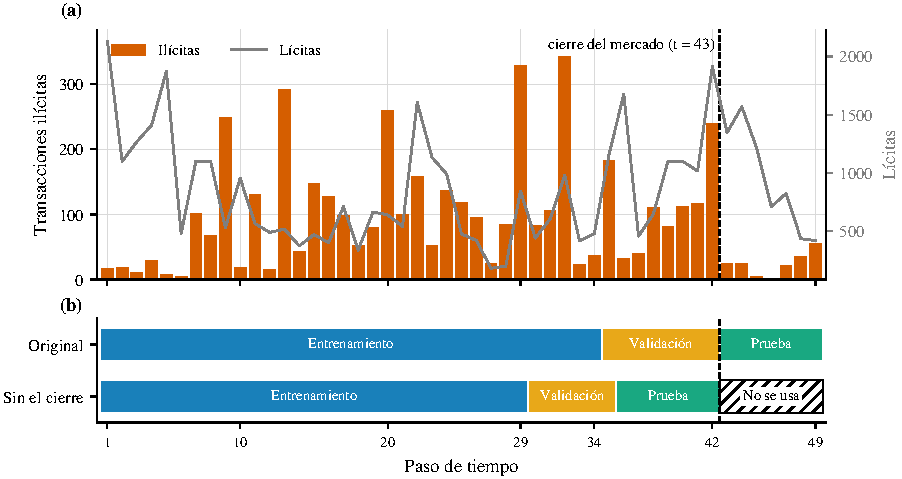
\includegraphics[width=\textwidth]{particion_temporal}
\caption{(a) Transacciones ilícitas (barras) y lícitas (línea) por paso de tiempo en Elliptic.
La línea discontinua marca el cierre del mercado ilegal en el paso 43. (b) Partición original
y partición sin el cierre usada en el estudio principal; en esta última los pasos 43 a 49 no
se usan.}
\label{fig:particion}
\end{figure}

\begin{table}[ht]
\centering
\caption{Transacciones por parte de cada partición. Negativas son lícitas más sin etiqueta;
la razón es negativas por cada ilícita.}
\label{tab:particion}
\small
% Generado por tesis_v4/scripts/analisis.py. No editar a mano.
\begin{tabular}{llrrrr}
\toprule
Partición & Parte & Pasos & Ilícitas & Negativas & Razón \\
\midrule
Original & Entrenamiento & 1 a 34 & 3.462 & 132.803 & 1:38{,}4 \\
 & Validación & 35 a 42 & 914 & 36.906 & 1:40{,}4 \\
 & Prueba & 43 a 49 & 169 & 29.515 & 1:174{,}6 \\
\midrule
Sin el cierre & Entrenamiento & 1 a 29 & 2.871 & 117.933 & 1:41{,}1 \\
 & Validación & 30 a 35 & 773 & 20.195 & 1:26{,}1 \\
 & Prueba & 36 a 42 & 732 & 31.581 & 1:43{,}1 \\
\bottomrule
\end{tabular}

\end{table}

La partición tiene tres costos que conviene declarar. Primero, el entrenamiento dispone de
2.871 transacciones ilícitas en lugar de 3.462, es decir, 591 menos que con la partición
habitual. Segundo, los cortes en los pasos 29 y 35 los escogieron los autores para que
validación y prueba tuvieran cada una cerca de una sexta parte de las ilícitas anteriores al
cierre; no responden a un criterio externo. Tercero, la prueba ya no mide la capacidad del
modelo para adaptarse a un cambio drástico del mercado, sino su desempeño en un periodo
posterior al entrenamiento pero en condiciones parecidas. Esta tesis no estudia la adaptación
a ese cambio, sino la estabilidad de las explicaciones, y para ello necesita modelos que
detecten de verdad.

\section{Escenarios de desbalance}\label{sec:escenarios}

El nivel de desbalance se modifica solo en el entrenamiento; validación y prueba conservan
siempre su proporción real. Los escenarios principales protegen la señal del fraude: no quitan
transacciones ilícitas, sino que submuestrean las negativas o sobremuestrean las ilícitas. Las
negativas se submuestrean de forma estratificada, conservando la misma mezcla de lícitas y sin
etiqueta que en el escenario nativo, con una semilla de datos fija (2026) que es distinta de la
semilla del modelo. Submuestrear significa sacar transacciones de la función de pérdida, no
del grafo: las transacciones descartadas siguen transmitiendo información a sus vecinas.

\begin{itemize}
  \item \textbf{Nativo (1:41,1).} Las 2.871 ilícitas y las 117.933 negativas del entrenamiento.
  \item \textbf{1:10 y 1:20.} Las 2.871 ilícitas y 28.710 o 57.420 negativas.
  \item \textbf{1:10 con SMOTE.} Las 2.871 ilícitas, 2.871 ilícitas sintéticas y 57.420
        negativas. Cada sintética interpola los atributos de una ilícita y de una de sus
        vecinas más cercanas en el espacio de atributos \cite{Chawla2002SMOTE}, se añade al
        grafo en el mismo paso de tiempo y hereda las aristas de la ilícita de la que parte.
  \item \textbf{1:100 y 1:200.} Escenarios de estrés solicitados por el director para forzar el
        desbalance más allá del real. Como el nativo ya usa todas las negativas, la única forma
        de llegar a esas razones es quitar ilícitas: se conservan 1.179 y 589 ilícitas, con
        las 117.933 negativas.
\end{itemize}

Los escenarios de estrés cambian dos cosas a la vez, la proporción y la cantidad absoluta de
ejemplos ilícitos, por lo que sus resultados se analizan junto a los principales pero se
interpretan con esa salvedad.

\section{Modelos y entrenamiento}\label{sec:entrenamiento}

Se entrenan cuatro arquitecturas de GNN para clasificar nodos: GCN \cite{Kipf2017GCN},
GraphSAGE \cite{Hamilton2017GraphSAGE}, GAT \cite{Velickovic2018GAT} y TAGCN
\cite{Du2017TAGCN}, descritas en la Sección \ref{sec:gnn}. Todas reciben el grafo completo y
producen una probabilidad de que cada transacción sea ilícita.

\textbf{Compensación del desbalance.} Se comparan tres funciones de pérdida (Sección
\ref{sec:desbalance}): entropía cruzada sin ajuste; entropía cruzada con pesos por clase
inversamente proporcionales a su frecuencia en el entrenamiento, de modo que cada clase aporta
la mitad de la pérdida total; y \textit{focal loss} \cite{Lin2020Focal} con $\gamma = 2$ y
$\alpha = 0{,}75$ como peso de la clase ilícita.

\textbf{Búsqueda de hiperparámetros.} Para cada combinación de arquitectura, escenario y
pérdida se hace una búsqueda bayesiana de 8 ensayos que maximiza el PR-AUC de validación.
El primer ensayo usa valores tomados de la literatura y los siguientes se proponen con un
estimador de Parzen. Cada ensayo entrena hasta 50 épocas, con parada temprana a las 10 épocas
sin mejora. El espacio es el mismo para las cuatro arquitecturas: dimensión oculta en
$\{64, 128, 148\}$, 2 o 3 capas, \textit{dropout} entre 0,1 y 0,5, tasa de aprendizaje entre
$10^{-4}$ y $10^{-2}$ y decaimiento de pesos entre $10^{-5}$ y $10^{-3}$, las dos últimas en
escala logarítmica. GAT busca además 2 o 4 cabezas de atención y TAGCN un orden de filtro $K$
entre 2 y 4. Por memoria, GAT se limita a 2 capas: con 148 dimensiones y 8 cabezas el
grafo completo no cabe en una GPU de 8~GB. Todas las arquitecturas reciben el mismo número de
ensayos y de épocas, para que la comparación no confunda arquitectura con presupuesto de
cómputo.

\textbf{Entrenamiento final y semillas.} Con los mejores hiperparámetros se entrena el modelo
final hasta 150 épocas con Adam, con parada temprana a las 20 épocas sin mejora del F1 de
validación. Esto se repite con tres semillas de modelo (42, 43 y 44); las semillas 43 y 44
reutilizan los hiperparámetros encontrados con la 42, de modo que la diferencia entre semillas
refleja solo la aleatoriedad del entrenamiento. Los hiperparámetros elegidos se listan en el Anexo
\ref{anx:tablas}. La búsqueda prefirió para TAGCN siempre 128 dimensiones y 3 capas, con órdenes
de filtro de 2 a 4, y para GAT siempre 2 capas; GraphSAGE alternó entre 2 y 3 capas y GCN eligió
casi siempre 2. El cálculo en GPU no es determinista a nivel de
pesos, porque las sumas de mensajes usan operaciones atómicas, lo que se suma a esa
aleatoriedad.

\textbf{Evaluación del rendimiento.} La métrica principal es el PR-AUC, el área bajo la curva
de precisión y exhaustividad, porque bajo un desbalance fuerte el ROC-AUC puede ser alto
aunque el modelo produzca muchas más falsas alarmas que aciertos \cite{Saito2015PR}. Se
reporta también el ROC-AUC. El umbral de decisión se fija en la validación, como el que
maximiza el F1, sin usar información de la prueba.

\textbf{Filtro de calidad.} Explicar un modelo que no aprendió no informa sobre el problema.
Por eso cada modelo se marca como aprobado si en validación, con umbral 0,5, alcanza un F1 de
al menos 0,30 y un coeficiente de Matthews \cite{Chicco2020MCC} de al menos 0,15. El filtro se
usa para interpretar los resultados, no para excluir modelos de la medición: todos los modelos
se explican, y los análisis principales se restringen a las arquitecturas que aprenden.

\section{Explicadores}\label{sec:explicadores}

\textbf{Transacciones explicadas.} Se explican las mismas 30 transacciones para todos los
modelos: 30 ilícitas de validación sorteadas con una semilla fija (1234) entre las 773
ilícitas de los pasos 30 a 35. Usar el mismo conjunto permite comparar explicaciones entre
modelos. Se explica la validación y no la prueba porque es el periodo con el que se
seleccionó el modelo y donde su comportamiento está mejor caracterizado. Las 30 transacciones son ilícitas, pero no todas son
verdaderos positivos para cada modelo: con el umbral de 0,5, los modelos con pesos por clase
aciertan en promedio entre 16,5 (TAGCN) y 22,3 (GCN) de ellas. Se explican todas, porque la
pregunta es cuán reproducible es la explicación de una predicción, sea acertada o no, y porque
restringirse a los aciertos de cada modelo impediría comparar modelos sobre las mismas
transacciones.

\textbf{Subgrafo receptivo.} Una GNN de $L$ capas solo usa, para predecir una transacción, la
información de sus vecinas a $L$ saltos o menos (a $L \cdot K$ saltos en TAGCN). Cada
explicación se calcula sobre ese subgrafo, y se verifica que la predicción del modelo en el
subgrafo coincida con la del grafo completo. Esto reduce la memoria de varios gigabytes a
unos pocos megabytes sin cambiar lo que se explica.

Se usan cinco explicadores, descritos en la Sección \ref{sec:xai}:

\begin{itemize}
  \item \textbf{GNNExplainer} \cite{Ying2019GNNExplainer}, que optimiza una máscara sobre las
        variables de los nodos del subgrafo durante 100 iteraciones con tasa de aprendizaje
        0,01. La importancia de cada variable es la media de su máscara sobre los nodos del
        subgrafo.
  \item \textbf{PGExplainer} \cite{Luo2020PGExplainer}, que entrena una red que asigna
        importancia a las aristas. Se entrena durante 100 épocas con 50 nodos, de los cuales al
        menos 25 son ilícitos. Como explica aristas y no variables, su estabilidad se reporta
        aparte.
  \item \textbf{Shapley por muestreo} \cite{Strumbelj2014Explaining, Castro2009Polynomial},
        que estima la contribución de cada variable promediando 50 permutaciones aleatorias;
        una variable ausente toma el valor medio de esa variable en el subgrafo.
  \item \textbf{Integrated Gradients} \cite{Sundararajan2017IG}, que integra el gradiente a lo
        largo del camino recto entre una referencia y la transacción, con 100 pasos. La
        referencia es la mediana del entrenamiento, que tras el escalado es el vector cero. Es
        determinista.
  \item \textbf{Expected Gradients} \cite{Erion2021Expected}, que promedia Integrated
        Gradients sobre 200 referencias tomadas al azar de 5.000 transacciones negativas del
        entrenamiento.
\end{itemize}

Ninguno de los explicadores de variables se entrena previamente: los dos de gradiente y el de
Shapley se aplican directamente al modelo, y GNNExplainer optimiza una máscara nueva para cada
transacción. Solo PGExplainer tiene una fase de entrenamiento propia.

\textbf{Réplicas.} Cada explicador se ejecuta cinco veces sobre cada transacción y cada modelo,
con semillas distintas. La estabilidad mide cuánto se parecen esas cinco explicaciones.

\subsection*{Detalles de implementación}

Los modelos y los explicadores se implementaron con PyTorch 2.6 y PyTorch Geometric 2.7; la
búsqueda de hiperparámetros con Optuna 4.8; las métricas con scikit-learn 1.8 y las pruebas
estadísticas con SciPy 1.17. GNNExplainer y PGExplainer son las implementaciones de PyTorch
Geometric. GNNExplainer se configuró para producir una máscara por variable y por nodo
(\texttt{node\_mask\_type="attributes"}) y una máscara por arista, y explica la salida del
modelo, no la etiqueta verdadera. Dos parámetros por defecto de PGExplainer se modificaron
porque producían resultados inválidos en Elliptic: el coeficiente de tamaño de la máscara se
bajó de 0,05 a 0,005, porque con el valor por defecto la máscara colapsaba a cero en todas las
aristas, y la temperatura se fijó en 1 en lugar del esquema de 5 a 2, porque con este último
la pérdida desbordaba a valores no numéricos. Además, los 50 nodos con que se entrena
PGExplainer se toman solo entre los que reciben al menos una arista: cerca del 30~\% de los
nodos de entrenamiento no recibe ninguna, y en ellos la pérdida de PGExplainer no está definida.
Shapley por muestreo, Integrated Gradients y Expected Gradients son implementaciones propias
(\texttt{src/explainability/}).

\section{Medidas de estabilidad}\label{sec:medidas}

Sea $\mathbf{a}^{(r)} \in \mathbb{R}^{165}$ el vector de importancias que la réplica $r$
asigna a las variables de una transacción. La estabilidad de esa transacción es el promedio,
sobre los $\binom{5}{2} = 10$ pares de réplicas, de una medida de acuerdo $s$:
\begin{equation}
  E = \frac{1}{10} \sum_{r < r'} s\!\left(\mathbf{a}^{(r)}, \mathbf{a}^{(r')}\right),
\end{equation}
y la estabilidad de un modelo es el promedio de $E$ sobre las 30 transacciones. Se usan tres
medidas de acuerdo:

\begin{description}
  \item[Spearman global (principal).] La correlación de rangos de Spearman
        \cite{Spearman1904} entre los dos vectores completos de 165 importancias. Es la medida
        más usada en la literatura y permite comparar con otros trabajos.
  \item[Spearman sobre las variables distintas de cero.] La misma correlación, calculada solo
        sobre las variables cuyo valor en la transacción es distinto de cero.
  \item[Jaccard top-10.] El índice de Jaccard \cite{Jaccard1912} entre los conjuntos de las 10
        variables más importantes de cada réplica, $|A \cap B| / |A \cup B|$. Si las dos
        réplicas comparten $k$ de sus 10 variables, el índice vale $k / (20 - k)$: compartir
        3, 5 o 7 variables da 0,18, 0,33 y 0,54.
\end{description}

Las dos medidas adicionales responden a un artefacto que se detectó durante el estudio. Una
variable que vale cero recibe una importancia nula o casi nula de los cuatro explicadores de
variables, por razones distintas en cada uno: Integrated Gradients multiplica el gradiente por
la diferencia entre la variable y la referencia, que es cero; la máscara de GNNExplainer anula
las entradas sin gradiente; y en Shapley y Expected Gradients la referencia suele coincidir con
cero. Esas variables, cerca de la mitad, quedan siempre al final del orden en cualquier
réplica y en cualquier modelo, y el Spearman global cuenta su acuerdo como si fuera
información. El tamaño de ese efecto se puede calcular. Si dos explicaciones solo coinciden en
dejar empatadas al final las variables nulas de la transacción y ordenan las demás al azar, su
correlación de Spearman media sobre las 30 transacciones es 0,81 (entre 0,54 y 0,86 según la
transacción, porque la fracción de variables nulas va del 23~\% al 50~\%). Ese es el piso que la
medida principal da sin que las explicaciones compartan nada sobre las variables que sí
importan (\texttt{tesis\_v4/scripts/piso\_spearman.py}).
El Spearman sobre las variables distintas de cero elimina el bloque, y el Jaccard top-10 solo
mira las variables que el analista vería primero.

Además de la estabilidad entre réplicas de un mismo modelo, se mide el acuerdo entre las
explicaciones medias de dos modelos distintos sobre las mismas transacciones: entre semillas,
entre escenarios, entre arquitecturas y entre explicadores.

\section{Control de pesos aleatorios}\label{sec:control}

Una explicación estable no es necesariamente una explicación del modelo. Si el explicador
dependiera solo de los datos de la transacción, daría el mismo resultado con cualquier modelo.
Para comprobarlo se aplica la prueba de aleatorización de parámetros de Adebayo et al.
\cite{Adebayo2018Sanity}: para cada arquitectura y semilla, en el escenario nativo con pesos por
clase (12 modelos), se explican las mismas 30 transacciones con el modelo entrenado y con dos
redes de la misma arquitectura e hiperparámetros pero con pesos aleatorios, sin entrenar. Se
reporta el acuerdo entre la explicación del modelo entrenado y la de la red aleatoria. Si ese
acuerdo es tan alto como la estabilidad entre réplicas, el orden de las variables no depende
de lo que el modelo aprendió.

\section{Análisis estadístico}\label{sec:estadistica}

La unidad independiente es el modelo entrenado, es decir, una arquitectura con una semilla.
Los modelos de una misma semilla en distintos escenarios parten de los mismos pesos iniciales y
de los mismos hiperparámetros, y sus explicaciones resultan casi idénticas (acuerdo de 0,96
entre escenarios con la misma semilla frente a 0,92 entre semillas). Tratarlos como
observaciones independientes inflaría la significancia, por lo que las pruebas se construyen
así:

\begin{description}
  \item[H1 (escenario).] Prueba de Friedman \cite{Friedman1937} con 9 bloques (3 arquitecturas
        que aprenden por 3 semillas) y 6 tratamientos (los escenarios), con pesos por clase. Se
        complementa con una prueba de equivalencia de dos pruebas unilaterales (TOST)
        \cite{Lakens2017TOST} entre el nativo y 1:200 con margen de 0,05: rechazar ambas
        hipótesis nulas indica que la diferencia, si existe, es menor que el margen.
  \item[H2 (arquitectura).] Prueba de Friedman con 3 bloques (las semillas) y 4 tratamientos
        (las arquitecturas), sobre la media de los cuatro escenarios principales con pesos por
        clase. Con tres bloques la prueba tiene poca potencia, por lo que se reporta además en
        cuántas semillas queda primera cada arquitectura.
  \item[H3 (compensación).] Prueba de signos pareada sobre 9 pares (arquitectura por semilla,
        media de los cuatro escenarios principales), de pesos por clase frente a
        \textit{focal loss} y frente a sin ajuste.
\end{description}

Los intervalos de confianza de las figuras se obtienen por \textit{bootstrap} sobre los
modelos \cite{Efron1979Bootstrap}. Todas las pruebas se repiten con las tres medidas de
estabilidad, y una conclusión se considera sólida solo si las tres coinciden.
